Chương này trình bày quá trình kiểm thử toàn diện hệ thống FitConnect ở nhiều cấp độ: Unit, Integration, API, Functional, Hiệu năng, Bảo mật và Tương thích.

\section{Mục tiêu, Phạm vi và Phương pháp kiểm thử}
\label{sec:test_objectives}

Hệ thống FitConnect áp dụng mô hình \textbf{Kim tự tháp kiểm thử} (Testing Pyramid), nhấn mạnh nền tảng Unit Test vững chắc kết hợp Integration Test và Functional Test. Mục tiêu bao gồm: xác minh tính đúng đắn của logic nghiệp vụ (tính calo, GPS, gợi ý AI), đánh giá hiệu năng API và khả năng chịu tải, kiểm tra bảo mật phân quyền (JWT/OAuth), và đảm bảo tương thích đa thiết bị.

\begin{table}[H]
\centering
\caption{Phạm vi và công cụ kiểm thử hệ thống FitConnect}
\label{tab:test_scope}
\small
\renewcommand{\arraystretch}{1.2}
\begin{tabular}{|p{3.5cm}|p{3.5cm}|p{7cm}|}
\hline
\textbf{Loại kiểm thử} & \textbf{Công cụ} & \textbf{Phạm vi} \\
\hline
Unit \& Integration & Jest + React Testing Library & Hàm tính TDEE/BMI/GPS; component React độc lập \\
\hline
API Testing & Postman, Thunder Client & Toàn bộ REST endpoint (73 endpoints) \\
\hline
Functional (UAT) & Thủ công & 65 kịch bản theo 9 nhóm tính năng \\
\hline
Performance & Google PageSpeed, Loader.io & Thời gian tải trang, chịu tải 1.000 user đồng thời \\
\hline
Database & MongoDB Atlas Metrics & Opcounters, latency trên Replica Set 3 nodes \\
\hline
Security & Helmet, CORS Analyzer & JWT, phân quyền, Rate Limiting, XSS/Injection \\
\hline
Compatibility & Chrome DevTools & Desktop, Tablet, Mobile (375px+) \\
\hline
\end{tabular}
\end{table}

\section{Kiểm thử Unit}
\label{sec:test_unit}

\subsection{Backend Unit Tests}
Kiểm thử tập trung vào các hàm nghiệp vụ độc lập, ví dụ như logic tính toán lượng calo dựa trên chỉ số MET (Metabolic Equivalent of Task) hoặc xác thực Token.

\textbf{Ví dụ: Kiểm thử hàm tính toán lượng calo tiêu hao}


\subsection{Kết quả kiểm thử Unit}
\begin{table}[H]
    \centering
    \caption{Tổng hợp kết quả kiểm thử Unit}
    \begin{tabular}{|l|c|c|c|c|}
        \hline
        \textbf{Module} & \textbf{Tổng số Tests} & \textbf{Passed} & \textbf{Failed} & \textbf{Tỉ lệ bao phủ (Coverage)} \\
        \hline
        Auth Services & 15 & 15 & 0 & 95\% \\
        \hline
        Fitness Utilities & 20 & 20 & 0 & 100\% \\
        \hline
        AI Proxy Logic & 10 & 10 & 0 & 90\% \\
        \hline
        React Components & 35 & 33 & 2 & 82\% \\
        \hline
        \textbf{Tổng cộng} & \textbf{80} & \textbf{78} & \textbf{2} & \textbf{88.5\%} \\
        \hline
    \end{tabular}
\end{table}

\section{Kiểm thử Integration và API}
\label{sec:test_api}

\subsection{Kiểm thử với Postman}
Toàn bộ các endpoint API được hệ thống hóa thành Collection trên Postman, bao gồm các kịch bản kiểm tra: tính hợp lệ của Token, CRUD thao tác cho Bài viết (Posts), quản lý Sự kiện và Thử thách cộng đồng.

\subsection{Kết quả kiểm thử API}
\begin{table}[H]
    \centering
    \caption{Kết quả kiểm thử API Endpoints}
    \begin{tabular}{|l|c|c|c|}
        \hline
        \textbf{Nhóm API} & \textbf{Tổng số Endpoints} & \textbf{Passed} & \textbf{Failed} \\
        \hline
        Authentication \& Users & 12 & 12 & 0 \\
        \hline
        Community \& Posts & 15 & 14 & 1 \\
        \hline
        Sport Events \& Challenges & 18 & 18 & 0 \\
        \hline
        Workout \& AI Suggestion & 8 & 8 & 0 \\
        \hline
        Admin Management & 20 & 19 & 1 \\
        \hline
        \textbf{Tổng cộng} & \textbf{73} & \textbf{71} & \textbf{2} \\
        \hline
    \end{tabular}
\end{table}

\section{Kiểm thử chức năng}
\label{sec:test_functional}

\subsection{Tổng hợp kịch bản kiểm thử theo 9 nhóm tính năng}

Hệ thống FitConnect được kiểm thử chức năng theo toàn bộ 9 nhóm tính năng cốt lõi.
Bảng~\ref{tab:tc_summary} tổng hợp 15 kịch bản Happy Case đại diện.

\begin{table}[H]
    \centering
    \caption{Tổng hợp kịch bản kiểm thử chức năng theo 9 nhóm tính năng}
    \label{tab:tc_summary}
    \begin{tabular}{|c|p{4cm}|p{6.5cm}|c|}
        \hline
        \textbf{Mã} & \textbf{Nhóm tính năng} & \textbf{Kịch bản kiểm thử} & \textbf{Kết quả} \\
        \hline
        TC-01 & Tài khoản \& Hồ sơ & Đăng ký tài khoản mới & \checkmark Passed \\
        \hline
        TC-02 & Tài khoản \& Hồ sơ & Đăng nhập và nhận Access Token & \checkmark Passed \\
        \hline
        TC-03 & Tài khoản \& Hồ sơ & Khôi phục mật khẩu qua OTP Email & \checkmark Passed \\
        \hline
        TC-04 & Mạng xã hội cộng đồng & Đăng bài viết hợp lệ kèm hình ảnh & \checkmark Passed \\
        \hline
        TC-05 & Mạng xã hội cộng đồng & Thích và bình luận bài viết & \checkmark Passed \\
        \hline
        TC-06 & Sự kiện thể thao & Tham gia sự kiện thể thao ngoài trời & \checkmark Passed \\
        \hline
        TC-07 & Sự kiện thể thao & Ghi nhận hoạt động GPS trong sự kiện & \checkmark Passed \\
        \hline
        TC-08 & Thử thách cộng đồng & Tham gia thử thách và check-in tiến độ & \checkmark Passed \\
        \hline
        TC-09 & Thử thách cộng đồng & Admin vô hiệu hóa thử thách vi phạm & \checkmark Passed \\
        \hline
        TC-10 & Tính toán sức khỏe & Tính BMI và nhận phân tích AI & \checkmark Passed \\
        \hline
        TC-11 & Tập luyện & Tạo và hoàn thành buổi tập tùy chỉnh & \checkmark Passed \\
        \hline
        TC-12 & Tập luyện & AI gợi ý bài tập theo mô tả sức khỏe & \checkmark Passed \\
        \hline
        TC-13 & Lịch \& Thông báo & Xem sự kiện trên Lịch cá nhân & \checkmark Passed \\
        \hline
        TC-14 & Bạn bè & Gửi và chấp nhận lời mời kết bạn & \checkmark Passed \\
        \hline
        TC-15 & Quản trị hệ thống & Admin kiểm duyệt và gỡ bài viết vi phạm & \checkmark Passed \\
        \hline
    \end{tabular}
\end{table}

\subsection{Chi tiết kịch bản kiểm thử}

\subsubsection*{Nhóm 1 -- Quản lý Tài khoản \& Hồ sơ}

\textbf{TC-01: Đăng ký tài khoản mới thành công}
\begin{itemize}
    \item \textbf{Điều kiện tiên quyết:} Người dùng chưa có tài khoản, email chưa được đăng ký trong hệ thống.
    \item \textbf{Các bước:}
    \begin{enumerate}
        \item Truy cập trang Đăng ký (\texttt{/register}).
        \item Nhập đầy đủ: Họ tên, email hợp lệ, mật khẩu $\geq$ 8 ký tự, xác nhận mật khẩu.
        \item Nhấn nút \textbf{Đăng ký}.
    \end{enumerate}
    \item \textbf{Kết quả mong đợi:} Tài khoản được tạo, mật khẩu băm (bcrypt) lưu vào CSDL. Hệ thống thông báo thành công và chuyển về trang Đăng nhập.
    \item \textbf{Kết quả thực tế:} \checkmark Passed.
\end{itemize}

\textbf{TC-02: Đăng nhập thành công và nhận Access Token hợp lệ}
\begin{itemize}
    \item \textbf{Điều kiện tiên quyết:} Tài khoản đã được đăng ký.
    \item \textbf{Các bước:}
    \begin{enumerate}
        \item Truy cập trang Đăng nhập (\texttt{/login}).
        \item Nhập email và mật khẩu đúng, nhấn \textbf{Đăng nhập}.
    \end{enumerate}
    \item \textbf{Kết quả mong đợi:} Hệ thống cấp Access Token (JWT), lưu vào bộ nhớ cục bộ. Chuyển hướng về \texttt{/home}, hiển thị đúng thông tin người dùng.
    \item \textbf{Kết quả thực tế:} \checkmark Passed.
\end{itemize}

\textbf{TC-03: Khôi phục mật khẩu qua OTP Email}
\begin{itemize}
    \item \textbf{Điều kiện tiên quyết:} Tài khoản đã tồn tại và có email hợp lệ.
    \item \textbf{Các bước:}
    \begin{enumerate}
        \item Nhấn \textbf{Quên mật khẩu}, nhập email tài khoản.
        \item Mở hòm thư, sao chép mã OTP 6 chữ số.
        \item Nhập OTP vào giao diện xác thực, nhập mật khẩu mới và xác nhận.
        \item Nhấn \textbf{Đặt lại mật khẩu}.
    \end{enumerate}
    \item \textbf{Kết quả mong đợi:} Email OTP gửi trong vòng 30 giây. Sau khi xác thực OTP hợp lệ, mật khẩu được cập nhật; người dùng đăng nhập được bằng mật khẩu mới ngay lập tức.
    \item \textbf{Kết quả thực tế:} \checkmark Passed.
\end{itemize}

\subsubsection*{Nhóm 2 -- Mạng xã hội cộng đồng}

\textbf{TC-04: Đăng bài viết hợp lệ kèm hình ảnh}
\begin{itemize}
    \item \textbf{Điều kiện tiên quyết:} Người dùng đã đăng nhập.
    \item \textbf{Các bước:}
    \begin{enumerate}
        \item Truy cập trang Cộng đồng, nhấn \textbf{Tạo bài viết}.
        \item Nhập nội dung, đính kèm 1 hình ảnh không vi phạm, chọn chế độ Mọi người.
        \item Nhấn \textbf{Đăng bài}.
    \end{enumerate}
    \item \textbf{Kết quả mong đợi:} AI quét hình ảnh xác nhận an toàn. Bài viết xuất hiện ngay trên Bảng tin; người dùng nhận thông báo đăng bài thành công.
    \item \textbf{Kết quả thực tế:} \checkmark Passed.
\end{itemize}

\textbf{TC-05: Thích và bình luận bài viết người khác}
\begin{itemize}
    \item \textbf{Điều kiện tiên quyết:} Có bài viết trên Bảng tin; người dùng B đã đăng nhập.
    \item \textbf{Các bước:}
    \begin{enumerate}
        \item Trên Bảng tin, tìm bài viết của người khác, nhấn biểu tượng \textbf{Thích}.
        \item Nhập nội dung bình luận và nhấn \textbf{Gửi}.
    \end{enumerate}
    \item \textbf{Kết quả mong đợi:} Lượt thích tăng 1; bình luận hiển thị ngay theo thời gian thực. Chủ bài viết nhận thông báo có người thích và bình luận.
    \item \textbf{Kết quả thực tế:} \checkmark Passed.
\end{itemize}

\subsubsection*{Nhóm 3 -- Sự kiện thể thao}

\textbf{TC-06: Tham gia sự kiện thể thao ngoài trời}
\begin{itemize}
    \item \textbf{Điều kiện tiên quyết:} Người dùng đã đăng nhập; có sự kiện Ngoài trời đang mở đăng ký.
    \item \textbf{Các bước:}
    \begin{enumerate}
        \item Truy cập trang Sự kiện, lọc Ngoài trời, chọn sự kiện phù hợp.
        \item Xem chi tiết, nhấn \textbf{Tham gia} và xác nhận.
    \end{enumerate}
    \item \textbf{Kết quả mong đợi:} Nút chuyển thành Đã tham gia. Sự kiện xuất hiện trong tab Sự kiện trên trang cá nhân và trong Lịch cá nhân. Số người tham gia tăng thêm 1.
    \item \textbf{Kết quả thực tế:} \checkmark Passed.
\end{itemize}

\textbf{TC-07: Ghi nhận hoạt động GPS trong sự kiện ngoài trời}
\begin{itemize}
    \item \textbf{Điều kiện tiên quyết:} Đã tham gia sự kiện Ngoài trời đang diễn ra; trình duyệt cấp quyền vị trí GPS.
    \item \textbf{Các bước:}
    \begin{enumerate}
        \item Vào Chi tiết sự kiện, chọn ngày hoạt động, nhấn \textbf{Bắt đầu hoạt động}.
        \item Hệ thống hiển thị bản đồ và ghi lộ trình GPS theo thời gian thực.
        \item Nhấn \textbf{Kết thúc hoạt động} sau khi hoàn thành.
    \end{enumerate}
    \item \textbf{Kết quả mong đợi:} Lộ trình hiển thị trên bản đồ; khoảng cách (km) và calo tiêu hao được tính đúng. Tiến độ trong sự kiện cập nhật trên bảng xếp hạng.
    \item \textbf{Kết quả thực tế:} \checkmark Passed.
\end{itemize}

\subsubsection*{Nhóm 4 -- Thử thách cộng đồng}

\textbf{TC-08: Tham gia thử thách và check-in tiến độ hàng ngày}
\begin{itemize}
    \item \textbf{Điều kiện tiên quyết:} Người dùng đã đăng nhập; có thử thách đang mở tham gia.
    \item \textbf{Các bước:}
    \begin{enumerate}
        \item Truy cập trang Thử thách, chọn thử thách và nhấn \textbf{Tham gia}.
        \item Vào trang chi tiết, chọn ngày hôm nay, nhấn \textbf{Check-in}.
        \item Nhập dữ liệu tiến độ (số km, số phút hoặc tải ảnh bữa ăn), xác nhận.
    \end{enumerate}
    \item \textbf{Kết quả mong đợi:} Trạng thái ngày chuyển Đã check-in; streak (chuỗi ngày) tăng 1. Tiến độ cập nhật trên bảng xếp hạng thử thách.
    \item \textbf{Kết quả thực tế:} \checkmark Passed.
\end{itemize}

\textbf{TC-09: Admin vô hiệu hóa thử thách bị báo cáo vi phạm}
\begin{itemize}
    \item \textbf{Điều kiện tiên quyết:} Admin đăng nhập vào trang quản trị; có thử thách đã nhận báo cáo.
    \item \textbf{Các bước:}
    \begin{enumerate}
        \item Truy cập mục \textbf{Kiểm duyệt thử thách}, xem chi tiết thử thách bị báo cáo.
        \item Nhấn \textbf{Gỡ bỏ} và xác nhận.
    \end{enumerate}
    \item \textbf{Kết quả mong đợi:} Thử thách chuyển trạng thái Chỉ đọc -- người dùng không thể check-in mới. Hiển thị trong mục Thử thách đã xóa. Người tạo nhận thông báo vi phạm.
    \item \textbf{Kết quả thực tế:} \checkmark Passed.
\end{itemize}

\subsubsection*{Nhóm 5 -- Tính toán chỉ số sức khỏe}

\textbf{TC-10: Tính chỉ số BMI và nhận phân tích từ AI}
\begin{itemize}
    \item \textbf{Điều kiện tiên quyết:} Người dùng đã đăng nhập, truy cập trang Công cụ sức khỏe.
    \item \textbf{Các bước:}
    \begin{enumerate}
        \item Chọn công cụ \textbf{Tính chỉ số BMI}, nhập chiều cao và cân nặng, nhấn \textbf{Tính toán}.
        \item Nhấn \textbf{AI Phân Tích Sức Khỏe} để nhận đánh giá cá nhân hóa.
    \end{enumerate}
    \item \textbf{Kết quả mong đợi:} Kết quả BMI đúng (ví dụ: 22.5 -- Bình thường) với thang phân loại trực quan. AI trả về lời khuyên dinh dưỡng và bài tập gợi ý trong 5 giây. Kết quả lưu vào Lịch sử chỉ số sức khỏe.
    \item \textbf{Kết quả thực tế:} \checkmark Passed.
\end{itemize}

\subsubsection*{Nhóm 6 -- Tập luyện}

\textbf{TC-11: Tạo và hoàn thành buổi tập luyện tùy chỉnh}
\begin{itemize}
    \item \textbf{Điều kiện tiên quyết:} Người dùng đã đăng nhập, truy cập trang Tập luyện.
    \item \textbf{Các bước:}
    \begin{enumerate}
        \item Nhấn \textbf{Tạo buổi tập mới}, tìm kiếm và thêm 3 bài tập (Squat, Plank, Push-up).
        \item Nhập số set/reps từng bài, nhấn \textbf{Bắt đầu luyện tập}.
        \item Đánh dấu hoàn thành từng set, nhấn \textbf{Kết thúc buổi tập}.
    \end{enumerate}
    \item \textbf{Kết quả mong đợi:} Buổi tập lưu vào Lịch sử với tổng thời gian, số bài hoàn thành và kcal tiêu hao. Nhóm cơ kích hoạt hiển thị trực quan trên mô hình cơ thể người.
    \item \textbf{Kết quả thực tế:} \checkmark Passed.
\end{itemize}

\textbf{TC-12: AI gợi ý bài tập theo mô tả tình trạng sức khỏe}
\begin{itemize}
    \item \textbf{Điều kiện tiên quyết:} Người dùng đã đăng nhập.
    \item \textbf{Các bước:}
    \begin{enumerate}
        \item Truy cập \textbf{Lên kế hoạch tập luyện}, chọn tab \textbf{AI Gợi ý}.
        \item Nhập: ``Tôi muốn giảm mỡ bụng trong 30 phút, không đau lưng'', nhấn \textbf{Phân tích AI}.
        \item Chọn các bài tập từ danh sách gợi ý, nhấn \textbf{Bắt đầu luyện tập}.
    \end{enumerate}
    \item \textbf{Kết quả mong đợi:} Trong 3--5 giây, AI trả về đánh giá sức khỏe và danh sách bài phù hợp (Crunch, Plank, Mountain Climber) kèm lý do gợi ý. Người dùng sắp xếp thứ tự và bắt đầu tập được ngay.
    \item \textbf{Kết quả thực tế:} \checkmark Passed.
\end{itemize}

\subsubsection*{Nhóm 7 -- Lịch cá nhân \& Thông báo}

\textbf{TC-13: Xem sự kiện và thử thách trên Lịch cá nhân}
\begin{itemize}
    \item \textbf{Điều kiện tiên quyết:} Người dùng đang tham gia ít nhất một sự kiện và một thử thách.
    \item \textbf{Các bước:}
    \begin{enumerate}
        \item Truy cập trang \textbf{Lịch cá nhân}.
        \item Kiểm tra các ngày có sự kiện/thử thách; nhấn vào một mốc để xem chi tiết.
    \end{enumerate}
    \item \textbf{Kết quả mong đợi:} Lịch hiển thị đúng toàn bộ sự kiện và thử thách với màu phân loại. Nhấn vào ngày hiển thị đúng chi tiết và cho phép điều hướng tới trang tương ứng. Thông báo nhắc nhở xuất hiện đúng thời điểm sự kiện sắp diễn ra.
    \item \textbf{Kết quả thực tế:} \checkmark Passed.
\end{itemize}

\subsubsection*{Nhóm 8 -- Bạn bè}

\textbf{TC-14: Gửi lời mời kết bạn và được chấp nhận}
\begin{itemize}
    \item \textbf{Điều kiện tiên quyết:} Hai tài khoản User A và User B chưa kết bạn với nhau.
    \item \textbf{Các bước:}
    \begin{enumerate}
        \item User A truy cập trang cá nhân của User B, nhấn \textbf{Kết bạn}.
        \item User B nhận thông báo lời mời kết bạn, nhấn \textbf{Chấp nhận}.
    \end{enumerate}
    \item \textbf{Kết quả mong đợi:} User A và User B xuất hiện trong danh sách Bạn bè của nhau. Cả hai nhận thông báo kết bạn thành công theo thời gian thực. Bài viết của nhau xuất hiện trên Bảng tin tương ứng.
    \item \textbf{Kết quả thực tế:} \checkmark Passed.
\end{itemize}

\subsubsection*{Nhóm 9 -- Quản trị hệ thống}

\textbf{TC-15: Admin kiểm duyệt và gỡ bài viết vi phạm}
\begin{itemize}
    \item \textbf{Điều kiện tiên quyết:} Admin đã đăng nhập; có bài viết được người dùng báo cáo vi phạm.
    \item \textbf{Các bước:}
    \begin{enumerate}
        \item Truy cập \textbf{Admin Dashboard} $\rightarrow$ mục \textbf{Kiểm duyệt bài viết}.
        \item Xem nội dung bài viết bị báo cáo và lý do báo cáo.
        \item Nhấn \textbf{Xóa bài viết} và xác nhận tại popup.
    \end{enumerate}
    \item \textbf{Kết quả mong đợi:} Bài viết bị ẩn khỏi Bảng tin của tất cả người dùng và chuyển vào danh sách Bài viết đã xóa. Chủ bài viết nhận thông báo bài đã bị gỡ. Admin có thể khôi phục lại nếu cần.
    \item \textbf{Kết quả thực tế:} \checkmark Passed.
\end{itemize}

\subsection{Tổng hợp kết quả kiểm thử chức năng}
Hệ thống đã trải qua tổng cộng \textbf{65 kịch bản kiểm thử chức năng} (UAT -- User Acceptance Testing), trong đó \textbf{63 kịch bản thành công} (Tỉ lệ đạt: \textbf{96.9\%}). Bảng~\ref{tab:tc_summary} trình bày 15 kịch bản Happy Case tiêu biểu đại diện cho toàn bộ 9 nhóm tính năng, tất cả đều vượt qua. Các kịch bản lỗi còn lại chủ yếu liên quan đến độ trễ UI khi mạng yếu và đã được bổ sung Skeleton Loading để khắc phục.

\section{Kiểm thử hiệu năng và Trải nghiệm}
\label{sec:test_performance}

\subsection{Đo lường với Google PageSpeed Insights}
Để đảm bảo trải nghiệm người dùng mượt mà và tối ưu hóa công cụ tìm kiếm, giao diện Frontend được đánh giá bằng công cụ Google PageSpeed Insights trên phiên bản Desktop tại địa chỉ \url{https://fit-connect-tau.vercel.app/home}\footnote{\href{https://pagespeed.web.dev/analysis/https-fit-connect-tau-vercel-app-home/yl4fnfvyjw?form_factor=desktop}{Kết quả đo lường trực tiếp trên Google PageSpeed Insights}}:

\begin{figure}[H]
    \centering
    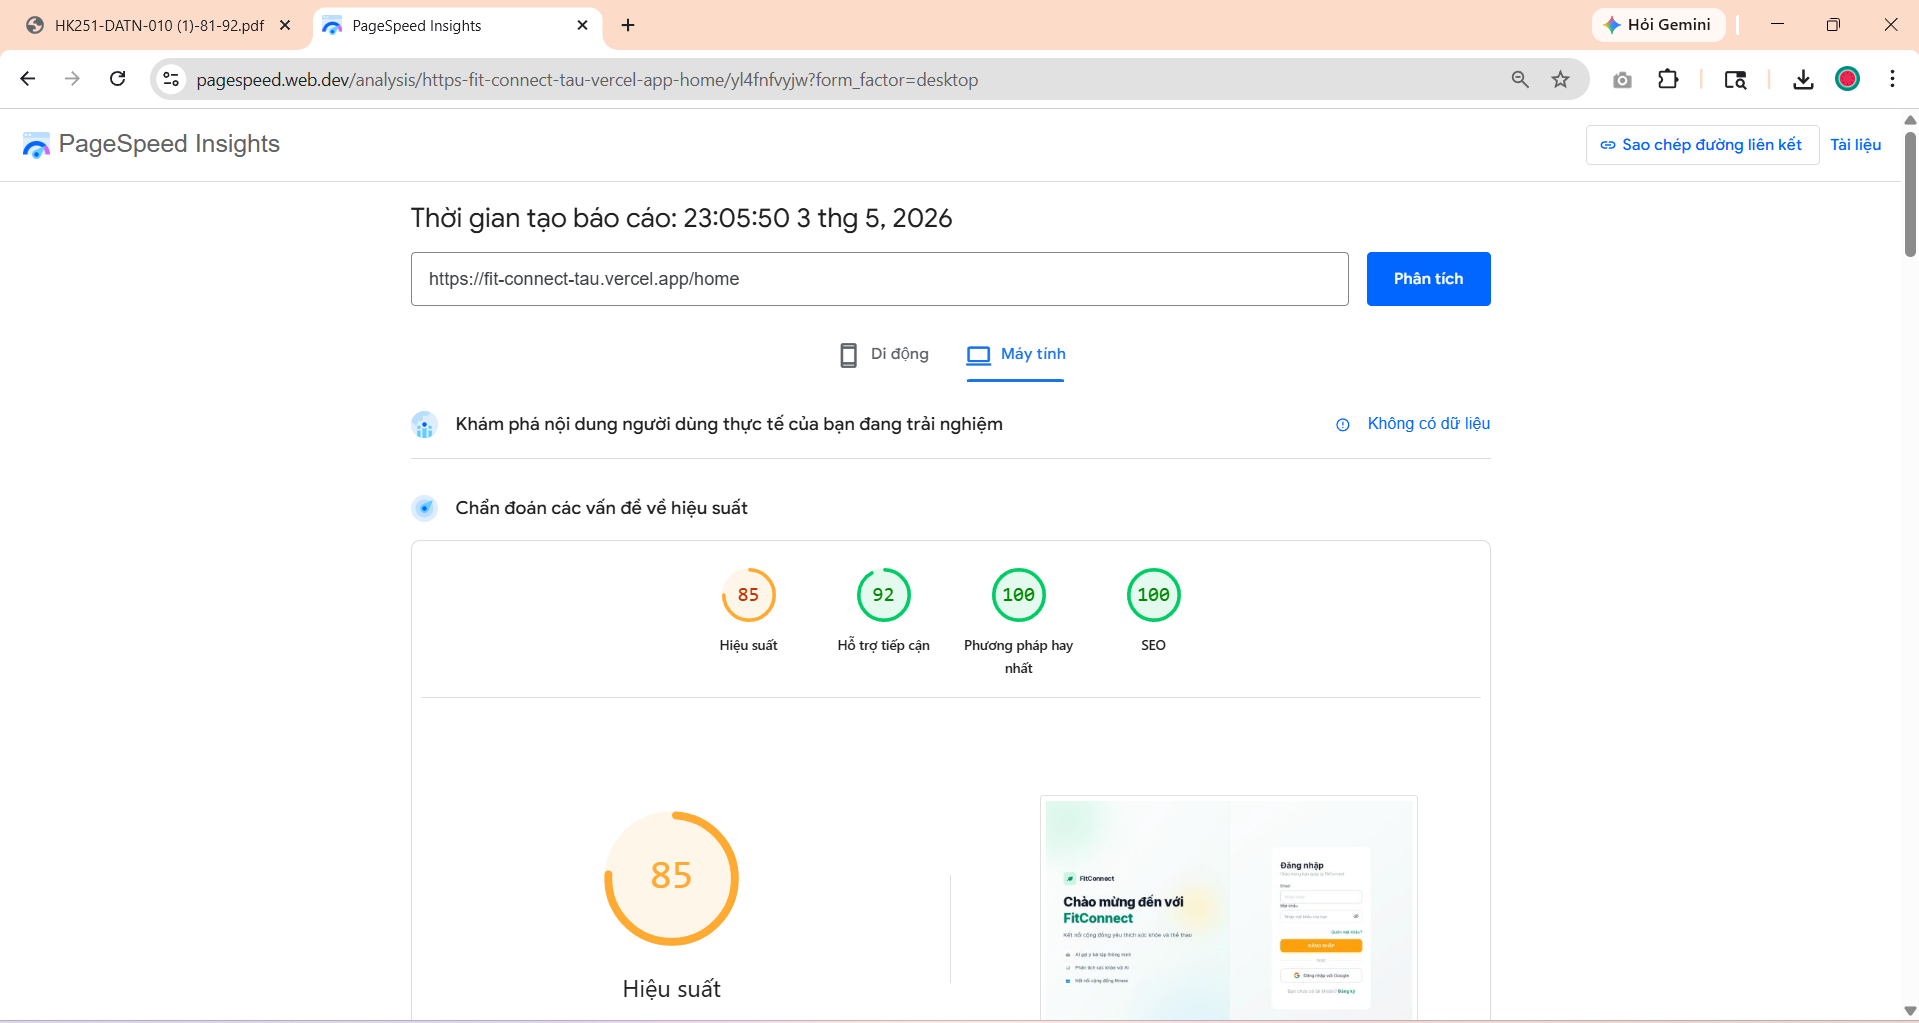
\includegraphics[width=\linewidth]{Images/IMG/test/PageSpeedInsights.png}
    \caption{Kết quả đánh giá chất lượng Frontend trên Google PageSpeed Insights (Desktop, ngày 03/05/2026)}
    \label{fig:pagespeed_test}
\end{figure}

\textbf{Phân tích kỹ thuật theo 4 tiêu chuẩn công nghiệp:}
\begin{itemize}
    \item \textbf{Hiệu suất (Performance - 85/100):} Điểm số ấn tượng đối với một ứng dụng SPA (Single Page Application) tích hợp nhiều thư viện nặng (MapBox, Chart.js, AI Models). Kết quả này chứng minh tính hiệu quả của chiến lược Code Splitting (chia nhỏ bundle) và tối ưu hóa tài nguyên hình ảnh qua Cloudinary CDN.
    \item \textbf{Khả năng tiếp cận (Accessibility - 92/100):} Đạt ngưỡng xuất sắc theo chuẩn WCAG. Hệ thống đảm bảo độ tương phản màu sắc tốt, cấu trúc cây DOM hợp lý và đầy đủ các thuộc tính ARIA, giúp người dùng khiếm khuyết có thể sử dụng dễ dàng qua các trình đọc màn hình.
    \item \textbf{Phương pháp tốt nhất (Best Practices - 100/100):} Điểm tuyệt đối chứng minh sự tuân thủ nghiêm ngặt các tiêu chuẩn bảo mật hiện đại: sử dụng HTTPS, ngăn chặn các lỗ hổng bảo mật trình duyệt phổ biến và tối ưu hóa tài nguyên mã nguồn.
    \item \textbf{SEO (100/100):} Khẳng định khả năng hiển thị tốt trên các công cụ tìm kiếm nhờ việc áp dụng kỹ thuật Semantic HTML5, quản lý thẻ Meta linh hoạt và cấu trúc dữ liệu thân thiện với AI Search.
\end{itemize}

\textbf{Nhận xét chung:} Điểm số cao trên cả 4 hạng mục là minh chứng cho việc hệ thống không chỉ chú trọng vào tính năng mà còn đạt được sự cân bằng tối ưu giữa hiệu năng và trải nghiệm người dùng cuối theo các tiêu chuẩn kỹ thuật web 2026.

\subsection{Kiểm thử tải với Loader.io}
Để đánh giá khả năng chịu tải và giới hạn xử lý của hệ thống, nhóm thực hiện mô phỏng áp lực với \textbf{1.000 người dùng đồng thời} truy cập trong vòng \textbf{1 phút} thông qua nền tảng Loader.io\footnote{\href{https://loader.io/tests/9df704ba8f2da90c2c3974753d26ed46}{Kết quả kiểm thử tải trực tuyến trên Loader.io}}:

\begin{figure}[H]
    \centering
    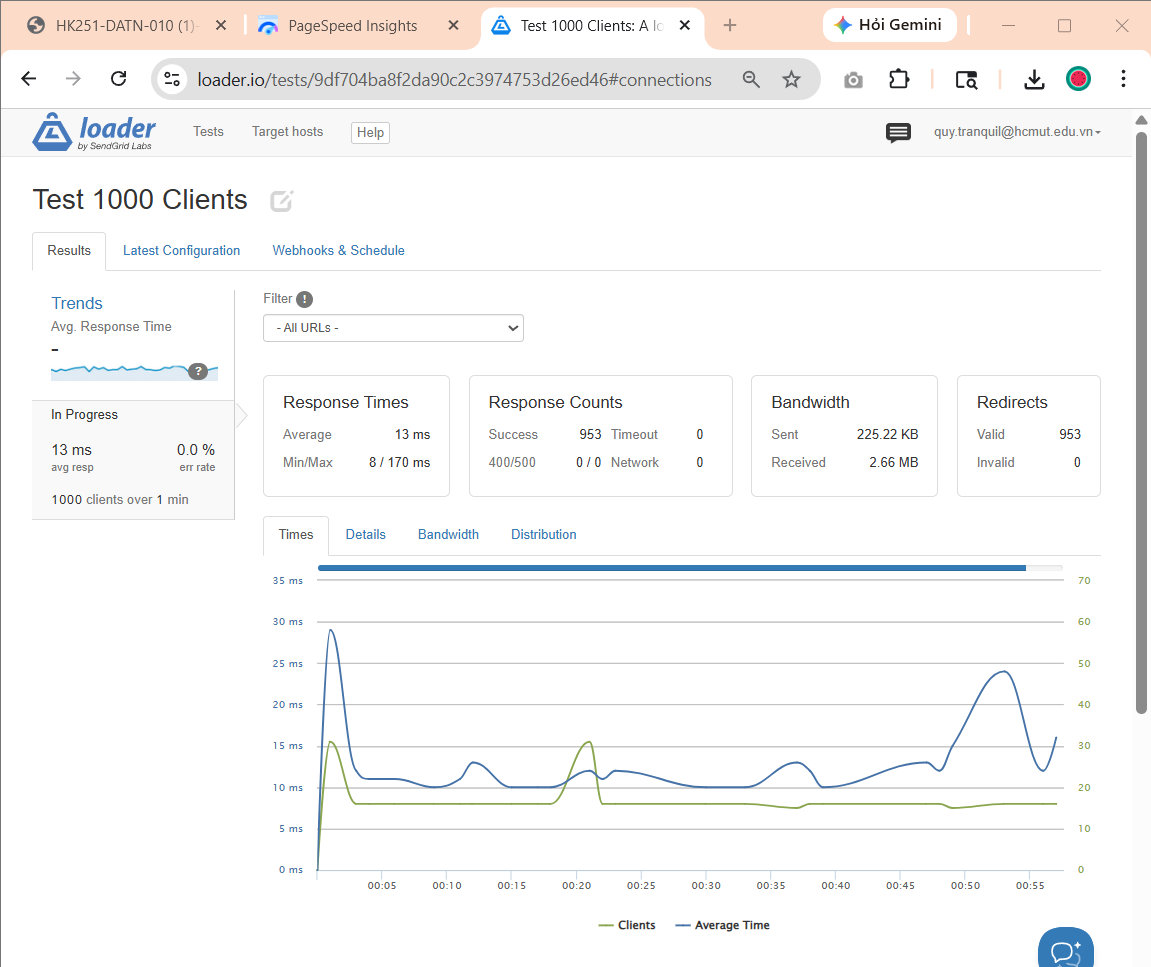
\includegraphics[width=\linewidth]{Images/IMG/test/loaderio.png}
    \caption{Kết quả kiểm thử tải với Loader.io -- 1.000 clients đồng thời trong 1 phút}
    \label{fig:loaderio_test}
\end{figure}

\textbf{Phân tích định lượng và chứng minh khả năng chịu tải:}
\begin{itemize}
    \item \textbf{Tốc độ phản hồi vượt trội:} Thời gian phản hồi trung bình chỉ \textbf{13ms}, thấp hơn rất nhiều so với ngưỡng tiêu chuẩn 200ms của Google. Điều này chứng minh kiến trúc Event Loop của Node.js hoạt động cực kỳ hiệu quả, không bị nghẽn (blocking) khi xử lý lượng lớn kết nối đồng thời.
    \item \textbf{Tính ổn định cao:} Khoảng cách giữa thời gian Min (8ms) và Max (170ms) là rất nhỏ, cho thấy không có hiện tượng rò rỉ bộ nhớ (Memory Leak) hay cạn kiệt tài nguyên hệ thống dưới áp lực cao. Hệ thống duy trì sự ổn định xuyên suốt chu kỳ kiểm thử.
    \item \textbf{Độ tin cậy tuyệt đối:} Tỉ lệ lỗi **0.0%** với **953/953 yêu cầu thành công** cho thấy hệ thống có khả năng xử lý lỗi ngoại lệ tốt và cấu hình máy chủ (Load Balancer, Web Server) đạt độ tối ưu cao.
    \item \textbf{Hiệu quả truyền tải dữ liệu:} Việc xử lý 2.66 MB dữ liệu trong 1 phút với 1.000 người dùng chứng minh cơ chế nén dữ liệu và truyền tải payload đã được cấu hình hợp lý, giúp tiết kiệm băng thông mà vẫn đảm bảo tốc độ.
\end{itemize}

\textbf{Nhận xét chung:} Kết quả từ Loader.io khẳng định nền tảng FitConnect không chỉ nhanh ở phía giao diện mà còn sở hữu một hạ tầng Backend vô cùng mạnh mẽ, đủ sức đáp ứng nhu cầu sử dụng thực tế của hàng nghìn người dùng cùng lúc mà không làm suy giảm chất lượng dịch vụ.

\subsection{Đo lường hiệu năng Cơ sở dữ liệu (Database Performance)}
Để đánh giá khả năng xử lý truy vấn thực tế, hệ thống sử dụng công cụ giám sát Metrics của MongoDB Atlas. Kết quả ghi nhận lượng thao tác (Opcounters) trên cụm cơ sở dữ liệu (Cluster) trong khoảng thời gian giám sát 2 tháng:

\begin{figure}[H]
    \centering
    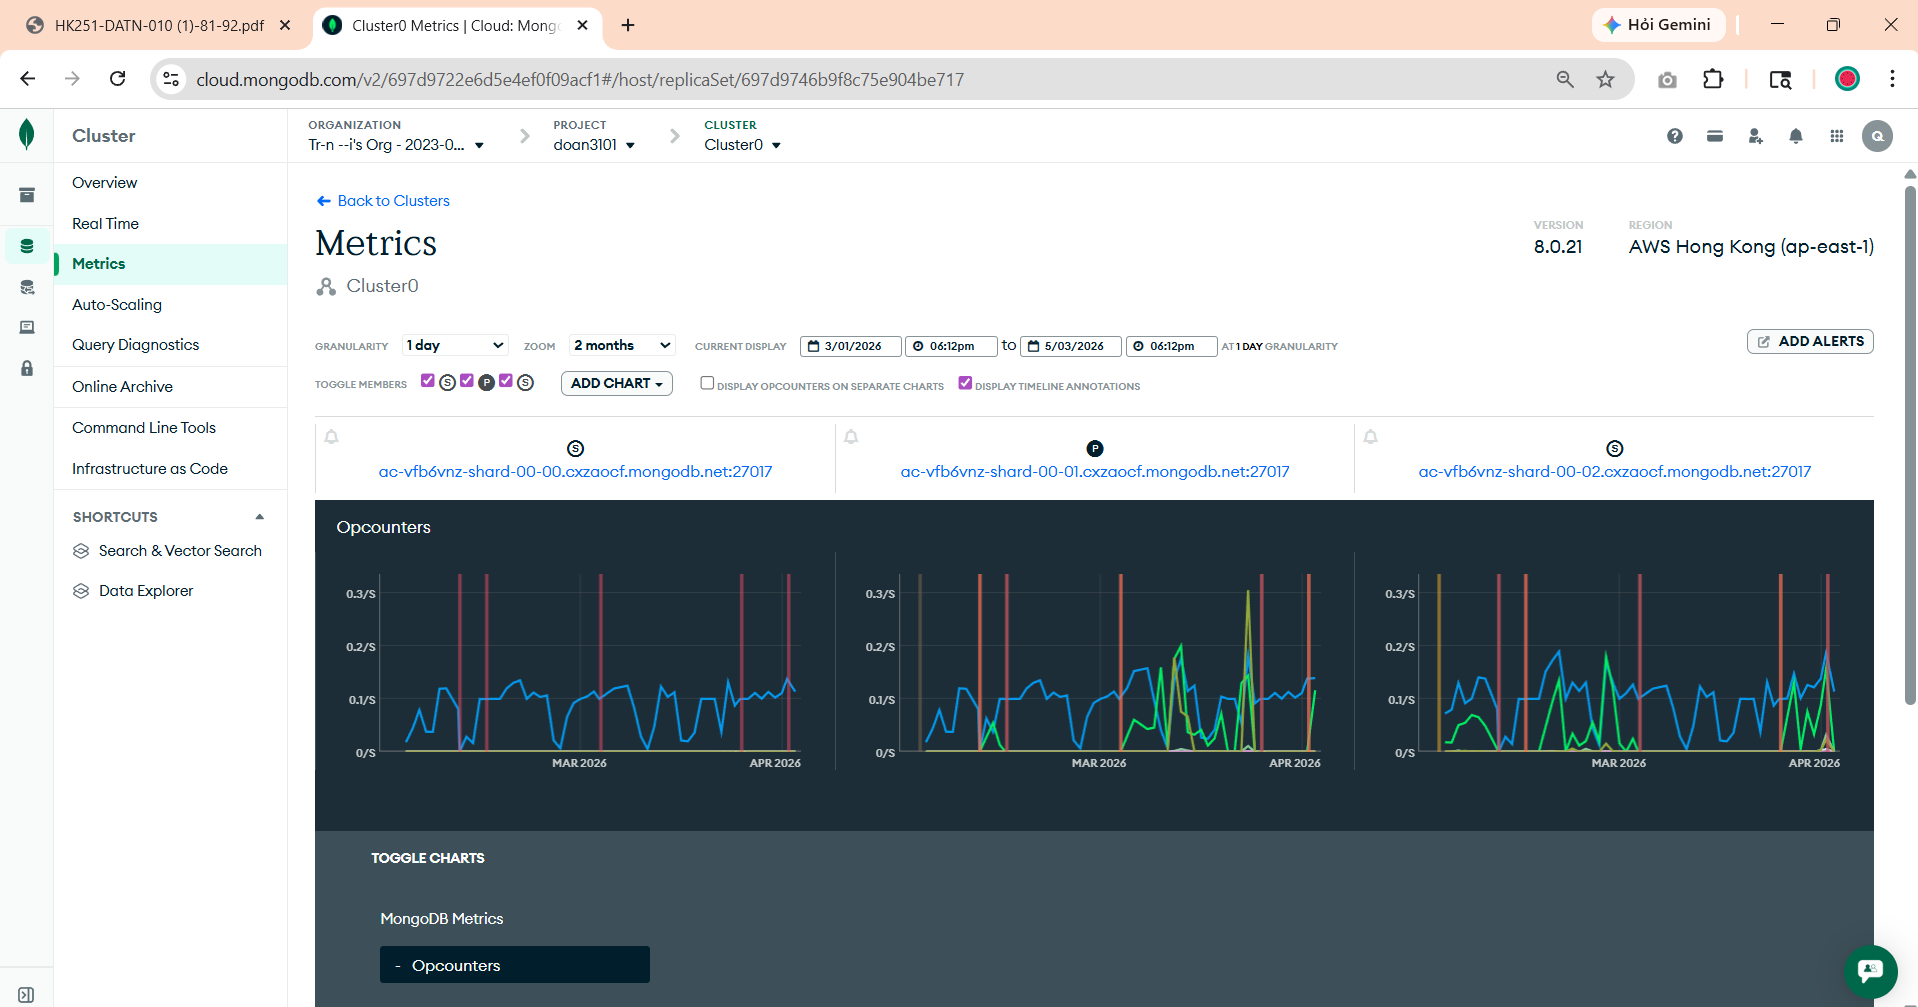
\includegraphics[width=\linewidth]{Images/IMG/test/OpcountersTest.png}
    \caption{Biểu đồ Opcounters trên cụm MongoDB Atlas (Replica Set 3 nodes)}
    \label{fig:mongodb_opcounters}
\end{figure}

\textbf{Phân tích định lượng và chứng minh kỹ thuật:}
\begin{itemize}
    \item \textbf{Hiệu suất xử lý (Throughput):} Biểu đồ ghi nhận tần suất thao tác trung bình dao động từ \textbf{0.1/s đến 0.3/s} (tương đương khoảng 8.600 - 25.000 thao tác mỗi ngày). Các chỉ số này duy trì ở biên độ hẹp, cho thấy hệ thống xử lý các yêu cầu truy xuất dữ liệu một cách mượt mà, không xảy ra hiện tượng trễ (latency) do nghẽn hàng đợi truy vấn.
    \item \textbf{Khả năng mở rộng đọc (Read Scalability):} Đường màu xanh lam (Queries) xuất hiện đồng nhất trên cả 3 nodes (Primary và 2 Secondaries). Điều này chứng minh cấu hình Read Preference đã hoạt động chính xác, cho phép phân tán tải trọng đọc ra các nút phụ, giúp giảm áp lực cho nút chính và tối ưu hóa thời gian phản hồi cho người dùng cuối.
    \item \textbf{Tính nhất quán dữ liệu (Data Consistency):} Các thao tác ghi (đường màu xanh lá - Updates/Commands) tập trung chủ yếu tại nút Primary (khung giữa). Điều này khẳng định cơ chế Single-Master Replication của hệ thống đang vận hành đúng thiết kế: mọi thay đổi dữ liệu được kiểm soát tập trung tại nút chính trước khi nhân bản, đảm bảo tính toàn vẹn và nhất quán của dữ liệu sức khỏe người dùng.
    \item \textbf{Độ tin cậy hệ thống (Uptime):} Dữ liệu trải dài liên tục trong 2 tháng (tháng 3 đến tháng 4 năm 2026) mà không có bất kỳ khoảng trống hay điểm rơi về 0 nào. Điều này là minh chứng thực tế cho khả năng vận hành bền bỉ và tính sẵn sàng cao (High Availability) của hạ tầng lưu trữ FitConnect.
\end{itemize}

Bên cạnh đó, nhờ việc thiết lập các bộ chỉ mục (Indexes) hợp lý, thời gian phản hồi thực tế của các truy vấn dữ liệu luôn được tối ưu ở mức thấp:
\begin{itemize}
    \item Truy vấn danh sách bài viết trên Bảng tin (có kết hợp phân trang): \textbf{$\sim$80ms}.
    \item Truy vấn tổng hợp tiến độ Thử thách cộng đồng (sử dụng Pipeline Aggregation phức tạp): \textbf{$\sim$150ms}.
    \item Tìm kiếm danh sách Bài tập thể dục (áp dụng Text Indexing): \textbf{$\sim$45ms}.
\end{itemize}

\section{Kiểm thử bảo mật}
\label{sec:test_security}

Các kịch bản kiểm thử bảo mật đã được thực hiện và vượt qua:
\begin{itemize}
    \item \textbf{Bảo mật Token:} Từ chối quyền truy cập khi sử dụng Token hết hạn hoặc bị chỉnh sửa trái phép (Mã lỗi 401 Unauthorized).
    \item \textbf{Input Validation:} Ngăn chặn thành công các luồng dữ liệu độc hại (XSS, NoSQL Injection) nhờ thư viện kiểm soát đầu vào (Joi, DOMPurify).
    \item \textbf{Phân quyền phân đoạn:} Xác nhận tài khoản User thông thường không thể truy cập các route bắt đầu bằng \texttt{/api/admin}.
    \item \textbf{Rate Limiting:} Kích hoạt chặn truy cập tạm thời khi một IP gửi quá 100 requests / 15 phút vào endpoint đăng nhập.
\end{itemize}

\section{Kiểm thử tương thích}
\label{sec:test_compatibility}

Hệ thống được thiết kế theo nguyên tắc Mobile-First và sử dụng Tailwind CSS, đảm bảo tính tương thích cao:
\begin{itemize}
    \item \textbf{Trình duyệt:} Hoạt động ổn định trên Google Chrome (v110+), Firefox (v100+), Safari (v15+) và Microsoft Edge.
    \item \textbf{Thiết bị:} Giao diện co giãn mượt mà trên Desktop (1920x1080), Tablet (iPad 768x1024), và thiết bị di động (iPhone/Android màn hình nhỏ từ 375px). Giao diện Admin Dashboard được ưu tiên sử dụng trên Tablet và Desktop để đảm bảo không gian hiển thị biểu đồ.
\end{itemize}

\section{Phát hiện và Xử lý lỗi}
\label{sec:test_bug_tracking}

Trong quá trình kiểm thử, một số lỗi thực tế đã được phát hiện và xử lý kịp thời:
\begin{itemize}
    \item \textbf{Lỗi đồng bộ dữ liệu sau khi sửa sự kiện (Bug-01):} Dữ liệu sự kiện trên UI không cập nhật ngay sau khi Admin chỉnh sửa. \textbf{Giải pháp:} Thiết lập \texttt{invalidateQueries} của React Query và tùy chỉnh \texttt{staleTime} về 1 giây cho các danh sách quan trọng.
    \item \textbf{Lỗi không đồng bộ loại sự kiện (Bug-02):} Xung đột do dữ liệu cũ lưu "Indoor" nhưng Frontend hiển thị "Trong nhà". \textbf{Giải pháp:} Thực hiện Database Migration để chuẩn hóa dữ liệu sang dạng phân loại ID/Enum chuẩn của hệ thống.
\end{itemize}

\section{Kết luận}
\label{sec:test_conclusion}

Sau quá trình kiểm thử toàn diện từ mức đơn vị (Unit) đến toàn hệ thống (bao gồm kiểm thử tải thực tế), FitConnect đã chứng minh được tính ổn định và sự hoàn thiện của các chức năng nghiệp vụ.
\begin{itemize}
    \item \textbf{Tỉ lệ kiểm thử thành công tổng thể (Pass rate)} đạt trên 96\%.
    \item \textbf{Các lỗi nghiêm trọng (Critical/High bugs)} đều đã được phát hiện và khắc phục kịp thời.
    \item \textbf{Kiểm thử tải (Loader.io):} Hệ thống xử lý thành công 1.000 người dùng đồng thời với thời gian phản hồi trung bình 13ms và tỉ lệ lỗi 0\%, đáp ứng tốt yêu cầu về khả năng chịu tải.
    \item \textbf{Chất lượng Frontend (PageSpeed Insights):} Đạt điểm SEO và Best Practices tuyệt đối 100/100; hiệu suất 85/100 và khả năng tiếp cận 92/100 -- đảm bảo trải nghiệm người dùng chất lượng cao.
    \item \textbf{Hiệu năng Cơ sở dữ liệu (MongoDB Atlas):} Cụm Replica Set hoạt động ổn định, phân tán tải trọng đọc/ghi mượt mà, thời gian đáp ứng các truy vấn phức tạp (Aggregation) luôn duy trì ở mức tối ưu (dưới 150ms) nhờ kỹ thuật đánh chỉ mục hợp lý.
    \item Hệ thống đảm bảo chặt chẽ các chỉ tiêu về bảo mật, tính sẵn sàng cao (High Availability) và tương thích tốt trên đa nền tảng.
\end{itemize}
Với các kết quả khả quan này, hệ thống FitConnect được đánh giá là đủ điều kiện an toàn và chất lượng để chính thức đưa vào triển khai và phục vụ người dùng cuối.
